\documentclass[twoside, addpoints, 12pt, letterpage]{exam}
\usepackage[utf8]{inputenc}

\usepackage{datetime,emptypage,calculus}
\newcommand{\ilf}[1]{$\displaystyle #1 $}

\begin{document}

\begin{coverpages}
\scshape
\centering
\rule{\textwidth}{1.6pt}\vspace*{-\baselineskip}\vspace*{2pt}
\rule{\textwidth}{0.4pt} % Thin horizontal rule
%reload: 123

\vspace{0.75\baselineskip}
    
    {\Huge MAT 272 Labs}
    
%\vspace{0.75\baselineskip}
%%% aa

\rule{\textwidth}{0.4pt}\vspace*{-\baselineskip}\vspace{3.2pt}
\rule{\textwidth}{1.6pt} % Thick horizontal ruleaaa

\vspace{0.75\baselineskip}

This is a collection of labs to be used during the \sem semester.

\vspace{3\baselineskip}

These labs have been typed and compiled by Ethan A. Smith using the \LaTeX\, typesetting language. Any questions, errata, or comments regarding these labs should be sent to \href{mailto:esmith845@cvcc.edu}{esmith845@cvcc.edu}.

%\vspace{3\baselineskip}


%These labs have been edited and proofread by Jonathan E. Loss.

\vspace{3\baselineskip}
This document was last updated \usdate\today.

\tableofcontents
\cleardoublepage
\end{coverpages}

%a1
\section{Calculus I Review}
\begin{questions}
\question Compute the derivative of the following functions.
\begin{multicols}{3}
\begin{parts}
\part $\sin(x)$ \\[16pt]
\part $\cos(x)$ \\[16pt]
\part $x^3$ \\[16pt]
\part $3x$ \\[16pt]
\part $e^x$ \\[16pt]
\part $\displaystyle\frac{1}{x}$ \\[16pt]
\part $\displaystyle \frac{1}{x^2}$ \\[16pt]
\part $x^\pi$ \\[16pt]
\part $\arctan(x)$ \\[16pt]
\end{parts}

\end{multicols}

\question Computer the derivative of the following expressions using derivative rules.
\begin{multicols}{2}
\begin{parts}
\part $\displaystyle 2\sin(x)+\cos(x)$ \\[1in]
\part $\displaystyle  e^{\sin(x)}$ \\[1in]
\part $\displaystyle \frac{x+3}{x^2-x}$ \\[1in]
\part $\tan(x)$ \\[1in]
\part $\sec(x)$ \\[1in]
\part $xe^x$ \\[1in]
\part $(2x+1)^9$ \\[1in]
\part $\sin(x)\cos(x^2)$ \\[1in]
\end{parts}
\end{multicols}

\newpage

\question Find $\displaystyle \frac{dy}{dx}$ as a function of $x$ and $y$ for the implicit curve:
\[xy+y^2+x^2=3.\]
\begin{solutionorbox}[2.5in]

\end{solutionorbox}

\question Find $\displaystyle \ddx{f(x)^{100}}$:
\begin{solutionorbox}[2.5in]

\end{solutionorbox}

\question Find $\displaystyle \ddx{\ln\lrp{f(x)}*g(x)}$
\begin{solutionorbox}[2.5in]

\end{solutionorbox}

\newpage

\question Calculate these basic anti-derivatives.
\begin{multicols}{3}
\begin{parts}
\part $\indefintnp{\sin(x)}$ \\[1in]
\part $\indefintnp{\cos(x)}$ \\[1in]
\part $\indefintnp{x^3}$ \\[1in]
\part $\indefintnp{}$ \\[1in]
\part $\indefintnp{e^x}$ \\[1in]
\part $\indefintnp{\frac{1}{x}}$ \\[1in]
\part $\indefintnp{\frac{1}{x^2}}$ \\[1in]
\part $\indefintnp{x^\pi}$ \\[1in]
\part $\indefintnp{\sec(x)\tan(x)}$ \\[1in]
\end{parts}

\end{multicols}

\question Calculate the definite integral using one of the Fundamental Theorems of Calculus.
\begin{parts}
\part $\defintp{2}{4}{x^2+1}$
\begin{solutionorbox}[1.5in]

\end{solutionorbox}

\part $\defintvarnp{-\frac{\pi}{4}}{\frac{\pi}{4}}{\sec^2{\theta}}{\theta}$
\begin{solutionorbox}[1.5in]

\end{solutionorbox}

\end{parts}

\newpage

\question Find the area between the curves $f(x)=2x$ and $g(x)=x^2$ on the interval $[0,2]$.
\begin{solutionorbox}[2.5in]

\end{solutionorbox}

\question Find the area between the curves $f(x)=\sin(x)$ and $g(x)=\cos(x)$ on the interval $\displaystyle \left[\frac{\pi}{4}, \frac{5\pi}{4}\right]$.
\begin{solutionorbox}[2.5in]

\end{solutionorbox}

\question Calculate $\displaystyle\ddx{\defintvarnp{x}{x^2}{e^{t^2}}{t}}$.
\begin{solutionorbox}[3in]

\end{solutionorbox}




\end{questions}\cleardoublepage

\section{u-Substitution}
\begin{questions}
\question Determine a $u$ to use to integrate the given indefinite integral. Do not actually solve the integral.
\begin{parts}

\part $\indefintnp{ \frac{\sqrt{1-\frac{1}{x}}}{x^2} }$
\begin{solutionorbox}[0.75in]

\end{solutionorbox}

\part $\indefintvarnp{ \frac{e^y}{3e^y-2} }{y}$
\begin{solutionorbox}[0.75in]

\end{solutionorbox}

\part $\indefintvarnp{ \theta^2e^{\theta^3} }{\theta}$
\begin{solutionorbox}[0.75in]

\end{solutionorbox}

\part $\indefintvarnp{ z\sqrt{2-7z} }{z}$
\begin{solutionorbox}[0.75in]

\end{solutionorbox}

\end{parts}

\question Evaluate the definite integral using the $u$-substitution with the given $u$.
\begin{parts}
\part $\defintnp{0}{2}{2x\sqrt{1+x^2}};\quad u=1+x^2$
\begin{solutionorbox}[2.5in]

\end{solutionorbox}

\newpage

\part $\defintnp{1}{4}{ \frac{e^{1/x}}{x^2} };\quad u=1/x$
\begin{solutionorbox}[2.5in]

\end{solutionorbox}

\part $\defintnp{0}{\ln(2)}{ \frac{e^{2x}}{3+e^{2x}} };\quad u=3+e^{2x}$
\begin{solutionorbox}[2.5in]

\end{solutionorbox}

\part $\defintnp{-\pi/4}{\pi/4}{ \tan(x) };\quad u=\cos(x)$
\begin{solutionorbox}[2.5in]

\end{solutionorbox}

\end{parts}

\newpage

\question Evaluate the definite or indefinite integral. Some questions may require $u$-substitution and some may simply require some algebra manipulation.
\begin{parts}

\part $\indefintnp{3x^2e^{x^3-2x^2+7}-4xe^{x^3-2x^2+7}}$
\begin{solutionorbox}[2.5in]

\end{solutionorbox}

\part $\indefintvarnp{ \frac{\ln(w)}{w} }{w}$
\begin{solutionorbox}[2.5in]

\end{solutionorbox}

\part $\defintvarnp{0}{\sqrt[3]{7}}{ y^2e^{y^3} }{y}$
\begin{solutionorbox}[2.5in]

\end{solutionorbox}

\newpage

\part $\indefintvarp{ \sqrt{1+\sqrt{\alpha}} }{\alpha}$
\begin{solutionorbox}[2.75in]
Let $u=\sqrt{1+\sqrt{\alpha}}$, then $\boxed{ \frac{4}{5}\lrp{\sqrt{1+\sqrt{\alpha}}}^5-\frac{4}{3}\lrp{\sqrt{1+\sqrt{\alpha}}}^3+C }$
\end{solutionorbox}

\part $\defintvarnp{-\pi/2}{\pi/2}{ \sin^3(\theta)\cos(\theta) }{\theta}$
\begin{solutionorbox}[2.75in]

\end{solutionorbox}

\part $\defintnp{0}{\pi/4}{ \frac{e^{\tan(x)}}{\cos^2(x)} }$
\begin{solutionorbox}[2.75in]

\end{solutionorbox}

\end{parts}


\end{questions}\cleardoublepage

\section{Integration by Parts}
\begin{questions}
\question Solve the following integral using the Tabular Method for repeated Integration by Parts.
\begin{parts}
\part $\indefintnp{x^3e^{4x}}$
\begin{solutionorbox}[4.00in]

\end{solutionorbox}

\part $\indefintnp{x^2\sin(5x)}$
\begin{solutionorbox}[4.00in]

\end{solutionorbox}
\end{parts}

\newpage

\question Evaluate the following integrals using integration by parts.
\begin{parts}

\part $\indefintnp{xe^{-2x}}$
\begin{solutionorbox}[4.25in]

\end{solutionorbox}

\part $\indefintvarnp{e^{2\theta}\cos(3\theta)}{\theta}$
\begin{solutionorbox}[4.25in]

\end{solutionorbox}

\part $\indefintnp{x^8\ln(x)}$
\begin{solutionorbox}[4.25in]

\end{solutionorbox}

\part $\defintnp{2}{e^2}{x^2\ln(x)}$
\begin{solutionorbox}[4.25in]

\end{solutionorbox}

\newpage

\part $\defintvarnp{0}{1}{e^{2y}\sin\lrp{e^{2y}}}{y}$
\begin{solutionorbox}[4.25in]

\end{solutionorbox}

\part $\defintvarnp{0}{4}{e^{\sqrt{w}}}{w}$
\begin{solutionorbox}[4.25in]
\[\FToC{0}{4}{2\sqrt{w}e^{\sqrt{w}-2e^{\sqrt{w}}}}\]
\end{solutionorbox}
\end{parts}



\end{questions}\cleardoublepage

\section{Partial Fractions and Algebraic Techniques}
\begin{questions}
\question Use find the partial fraction decomposition of the following rational expressions.
\begin{parts}
\part $\displaystyle \frac{12x-11}{x^2-x}$
\begin{solutionorbox}[3.75in]

\end{solutionorbox}

\part $\displaystyle \frac{z^2+20z-15}{z^3+4z^2-5z}$
\begin{solutionorbox}[3.75in]

\end{solutionorbox}

\end{parts}

\newpage

\question Evaluate the following integrals.
\begin{parts}
\part $\indefintnp{\frac{x^2+3}{x^3-2x^2+x}}$
\begin{solutionorbox}[4.25in]

\end{solutionorbox}

\part $\indefintnp{\frac{8}{x^3-2x^2-4x+8}}$
\begin{solutionorbox}[4.25in]

\end{solutionorbox}

\part $\indefintnp{\frac{2x+3}{x^2+4}}$
\begin{solutionorbox}[4.25in]

\end{solutionorbox}

\part Use the fact that $\displaystyle \sec(x)=\frac{\cos(x)}{1-\sin^2(x)}$ and partial fractions to find $\indefintvarnp{\sec{\theta}}{\theta}$.
\begin{solutionorbox}[4.25in]

\end{solutionorbox}

\newpage

\part $\indefintvarnp{\frac{\sin(\theta)}{\cos(\theta)+\cos^2(\theta)}}{\theta}$.
\begin{solutionorbox}[4.25in]

\end{solutionorbox}

\part $\indefintnp{\frac{e^x}{e^{2x}-4e^x}}$.
\begin{solutionorbox}[4.25in]

\end{solutionorbox}
\end{parts}



\end{questions}\cleardoublepage

\section{Trigonometric Integrals}
\begin{questions}
\question Use an appropriate trigonometric integral to evaluate the following integrals.
\begin{parts}
\part $\indefintnp{\sin^3(x)}$
\begin{solutionorbox}[4.25in]
\end{solutionorbox}

\part $\indefintnp{\cos^3(x)}$
\begin{solutionorbox}[4.00in]
\end{solutionorbox}

\newpage

\part $\indefintnp{\cos^4(2x)}$
\begin{solutionorbox}[4.5in]
\end{solutionorbox}

\part $\indefintnp{\sin^2(x)\cos^2(x)}$
\begin{solutionorbox}[4.5in]
\end{solutionorbox}

\newpage

\part $\indefintnp{\sin^3(x)\cos^5(x)}$
\begin{solutionorbox}[4.5in]
\end{solutionorbox}

\part $\indefintnp{\sin^4(5x)}$
\begin{solutionorbox}[4.5in]
\end{solutionorbox}

\newpage

\part $\indefintnp{12\sec^4(x)}$
\begin{solutionorbox}[4.5in]
\end{solutionorbox}

\part $\indefintnp{\tan^3(x)}$
\begin{solutionorbox}[4.5in]
\end{solutionorbox}

\newpage

\part $\indefintnp{\tan(x)\sec^3(x)}$
\begin{solutionorbox}[4.5in]
\end{solutionorbox}

\part $\indefintnp{\sqrt{\tan(x)}\sec^4(x)}$
\begin{solutionorbox}[4.5in]
\end{solutionorbox}

\end{parts}


\end{questions}\cleardoublepage

\section{Trigonometric Substitutions}
\begin{questions}
\question Solve the following integral using the appropriate trigonometric substitution.
\begin{parts}
\part $\indefintnp{\frac{1}{\sqrt{25-x^2}}}$
\begin{solutionorbox}[4.00in]

\end{solutionorbox}

\part $\indefintnp{\frac{x^2}{\sqrt{1-x^2}}}$
\begin{solutionorbox}[4.00in]

\end{solutionorbox}

\newpage

\part $\indefintnp{\frac{1}{\lrp{4-x^2}^{3/2}}}$
\begin{solutionorbox}[4.50in]

\end{solutionorbox}

\part $\indefintnp{\sqrt{\lrp{81+x^2}}}$
\begin{solutionorbox}[4.50in]

\end{solutionorbox}

\newpage

\part $\defintnp{\frac{1}{\sqrt{3}}}{1}{\frac{1}{x^2\sqrt{1+x^2}}}$
\begin{solutionorbox}[4.45in]

\end{solutionorbox}

\part $\defintnp{1}{2}{\frac{1}{x^2\sqrt{4-x^2}}}$
\begin{solutionorbox}[4.45in]

\end{solutionorbox}

\end{parts}

\question A total charge $Q$ is distributed uniformly on a line segment of length $2L$ along the $y$-axis. The $x$-component of the electric field at a point $(a,0)$ on the $x$-axis is given by 
\[E_x(a)=\frac{kQa}{2L}\defintvarnp{-L}{L}{\frac{1}{\lrp{a^2+y^2}^{3/2}}}{y},\]
where $k$ is a physical constant and $a>0$\footnote{A detailed derivation of this can be found at \url{http://newb.kettering.edu/wp/experientialcalculus/wp-content/uploads/sites/15/2017/05/the-electric-field-of-a-line-of-charge.pdf}.}.
\begin{parts}
\part Use a trigonometric substitution to find an explicit formula for $E_x(a)$.
\begin{solutionorbox}[5.25in]

\end{solutionorbox}

\part Let $\rho=\frac{Q}{2L}$ be the charge density on the line segement. Show that if $L\to\infty$, then $E_x(a)=\frac{2k\rho}{a}.$
\begin{solutionorbox}[1.75in]
\end{solutionorbox}

\end{parts}


\end{questions}\cleardoublepage

\section{Unit 1 Review Questions}
\begin{multicols}{3}
\begin{enumerate}
\item\ilf{\int t e^{t^2}\  dt}\vspace{-.2\baselineskip}
\item\ilf{\int t e^{2t}\  dt}\vspace{-.2\baselineskip}
\item\ilf{\int t^3 \cos(t^2)\ dt}
\item\ilf{\int \ln (x^3)\  dx}
\item\ilf{\int \frac{dx}{\sqrt{1-x}}}
\item\ilf{\int \sec (5\theta)\  d \theta}
\item\ilf{\int \sin^2 x\  dx }
\item\ilf{\int \cot (3\alpha)\  d\alpha}
\item\ilf{\int \cos^3 x\  dx}
\item\ilf{\int \sec^3 (2\phi)\  d\phi}
\item\ilf{\int \sqrt{4+7t}\,dt}
\item\ilf{\int \sqrt{4+7t^2}\,dt}
\item\ilf{\int \sqrt{1-6t^2}\,dt}
\item\ilf{\int t^2 \sqrt[3]{1-7t^3}\,dt}
\item\ilf{\int t^2 \sin (2t)\  dt }
\item\ilf{\int te^{-t^2}\  dt}
\item\ilf{\int \cos(\sqrt{t})\  dt}
\item\ilf{\int \sin^8 x \cos^5 x \ dx }
\item\ilf{\int e^x \cos 2x\  dx }
\item\ilf{\int x^5 \ln x\    dx }
\item\ilf{\int \sin 3x \cos 4x\  dx }
\item\ilf{\int \frac{x}{1+2x^2}\, dx}
\item\ilf{\int \frac{dx}{4+x^2} }
\item\ilf{\int \frac{dx}{1-x^2}}
\item\ilf{\int \frac{2x}{(x^2+1)(x-1)^2}\, dx }
\item\ilf{\int \frac{4t+1}{t^2+t-2}\, dt}
\item\ilf{\int \frac{u^2+11}{u^2+4u+5}\, du}
\end{enumerate}
\end{multicols}
Determine if the following improper integrals are convergent or divergent. If they are convergent, determine the value to which they converge.
\begin{multicols}{3}
\begin{enumerate}
\item \ilf{ \defintnp{2}{\infty}{\frac{2x}{x^2+1}} }
\item \ilf{ \defintnp{0}{\infty}{xe^{-x}} }
\item \ilf{ \defintnp{-\infty}{0}{\frac{1}{1+x^2}} }
\item \ilf{ \defintnp{3}{\infty}{\frac{1}{\sqrt{x}}} }
\item \ilf{ \defintnp{0}{\infty}{\frac{e^x}{e^{2x}+1}} }
\item \ilf{ \defintnp{4/\pi}{\infty}{\frac{1}{x^2}\sec^2\lrp{\frac{1}{x}}} }
\end{enumerate}
\end{multicols}\cleardoublepage

\section{Volumes by Slicing -- Part 1}
\setcounter{figure}{0}
\begin{questions}

\question Find the volume of the solid whose base is the region bounded by the semicircle $y=\sqrt{4-x^2}$ and the $x$-axis and whose cross sections through the solid perpendicular to the $x$-axis are squares. For a 3D graph, go to \url{https://sagecell.sagemath.org/?q=ixkvvn}.
\begin{figure}[hbt!]\centering
  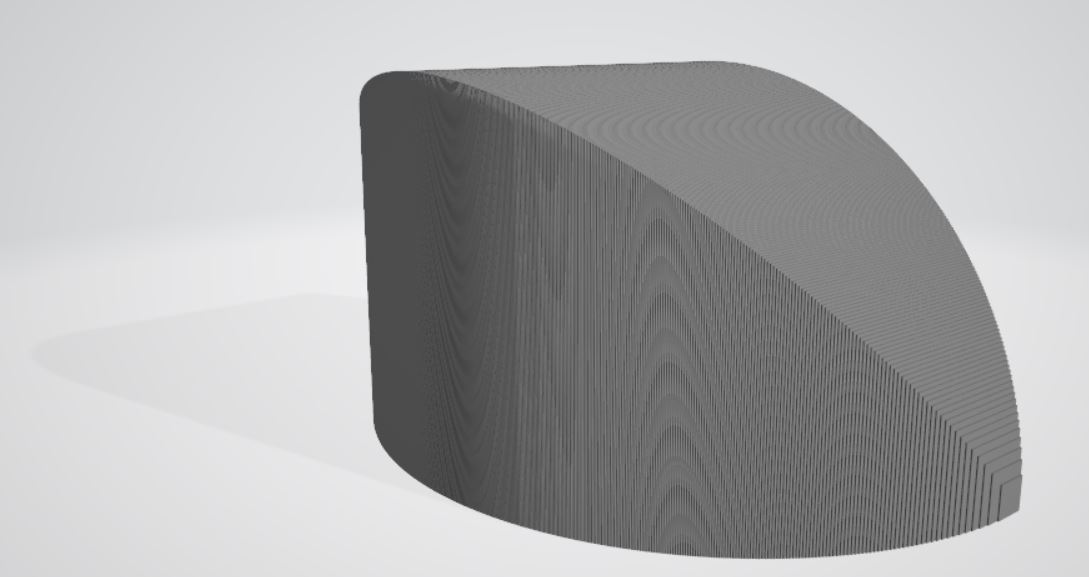
\includegraphics[scale=0.4]{plots/cross_section_squares.JPG}
  \caption{For a better view, go to \url{https://sagecell.sagemath.org/?q=rvlawp}.}
\end{figure}
\begin{solutionorbox}[6.0in]

\end{solutionorbox}

\newpage


\question Find the volume of the solid whose base is the region bounded by $y=x^2$ and the the line $y=4$ and whose cross sections are equilateral triangles parallel to the $x$-axis.
\begin{figure}[hbt!]\centering
  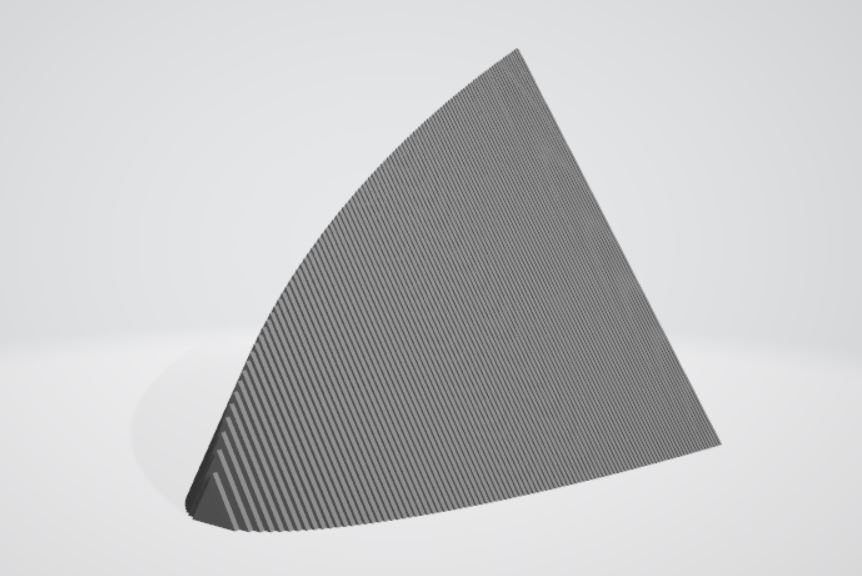
\includegraphics[scale=0.5]{plots/cross_section_triangles.JPG}
  \caption{For a better view, go to \url{https://sagecell.sagemath.org/?q=rvlawp}.}
\end{figure}

\begin{solutionorbox}[6.25in]

\end{solutionorbox}


\newpage


\question Let $R$ be the region bounded by the following curves. Use the disk (or washer) method to find the volume of the solid generated when $R$ is revolved about the $x$-axis.
\begin{parts}
\part $y=e^{-x}$ and the $x$-axis on the interval $[0,\ln(4)]$
  \begin{figure}[hbt!]\centering
    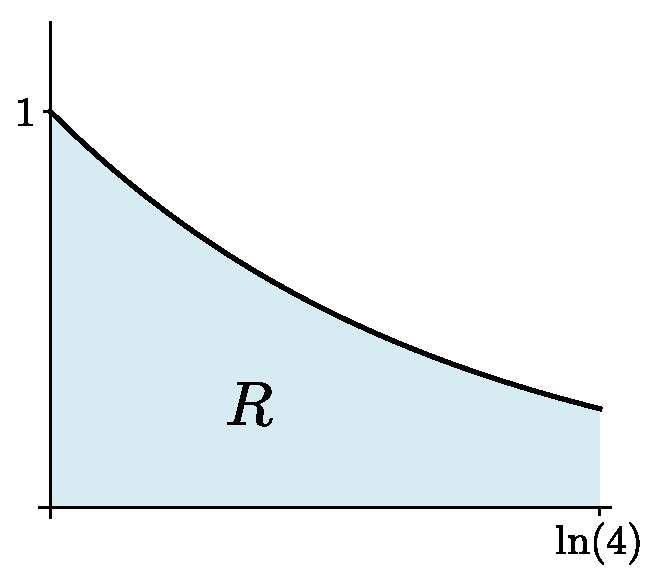
\includegraphics[scale=0.75]{plots/volumes_by_slicing_p1.pdf}
    \caption{Region bounded by $y=e^{-x}$ and the $x$-axis on the interval $[0, \,\ln(4)]$}
  \end{figure}

\begin{solutionorbox}[5.50in]

\end{solutionorbox}


\newpage


\part $y=x$ and $y=\sqrt[4]{x}$
  \begin{figure}[hbt!]\centering
    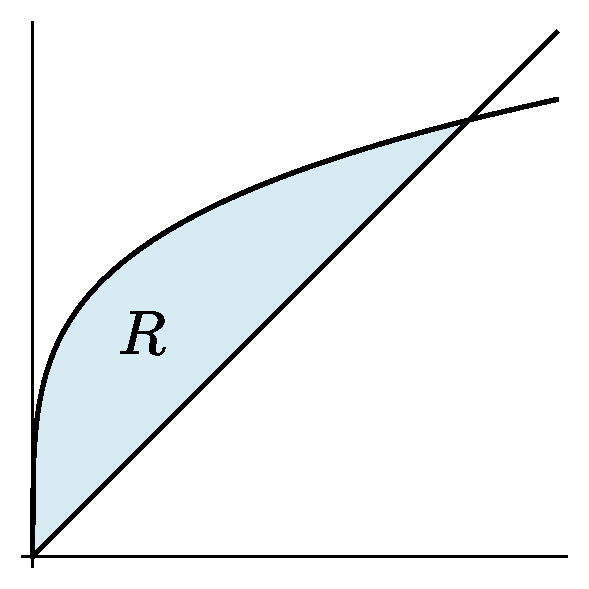
\includegraphics[scale=0.75]{plots/volumes_by_slicing_p2.pdf}
    \caption{Region bounded by $y=\sqrt[4]{x}$ and the $y=x$}
  \end{figure}

\begin{solutionorbox}[5.9in]

\end{solutionorbox}

\end{parts}


\newpage


\question Let $R$ be the region bounded by the following curves. Use the disk (or washer) method to find the volume of the solid generated when $R$ is revolved about the $y$-axis.
\begin{parts}

\part $y=16-x^2$ and the $x$-axis
  \begin{figure}[hbt!]\centering
    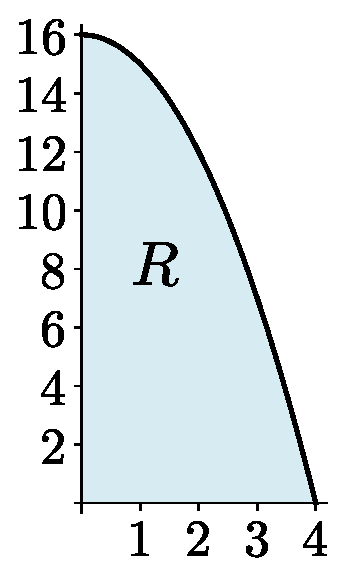
\includegraphics[scale=0.75]{plots/volumes_by_slicing_p4.pdf}
    \caption{Region bounded by $y=16-x^2$ and the $x$-axis}
  \end{figure}
  
\begin{solutionorbox}[5.4in]

\end{solutionorbox}

\newpage

\part $\displaystyle y=\frac{x}{2}$ and $y=\sqrt{x}$
  \begin{figure}[hbt!]\centering
    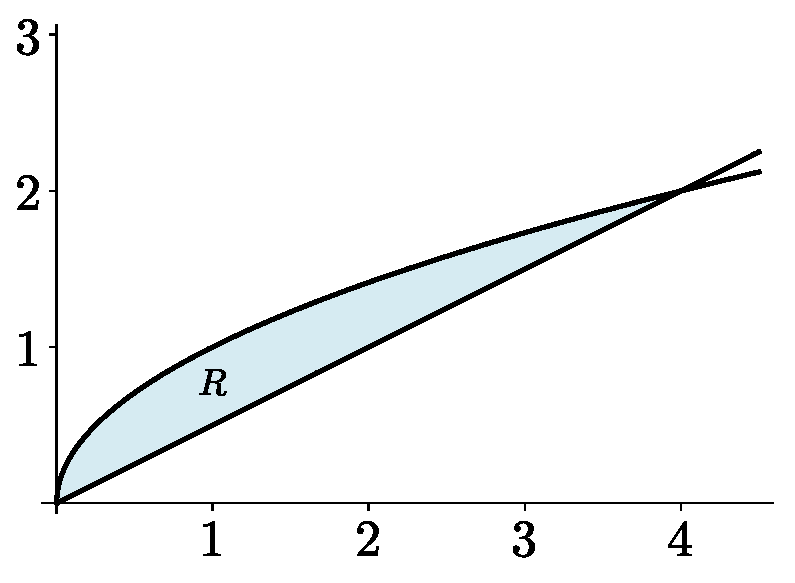
\includegraphics[scale=0.75]{plots/volumes_by_slicing_p5.pdf}
    \caption{Region bounded by $y=16-x^2$ and the $x$-axis}
  \end{figure}
  
\begin{solutionorbox}[6.00in]

\end{solutionorbox}

\end{parts}


\end{questions}\cleardoublepage

\section{Volumes by Slicing -- Part 2}
\setcounter{figure}{0}
\begin{questions}

\question Use disk (or washer) method to find the volume of the solid of revolution obtain by rotating the given region, $R$, about the specified axis of rotation.
\begin{parts}
\part $y=x+2$ and $y=x^2$ about the line $y=5$
  \begin{figure}[hbt!]\centering
    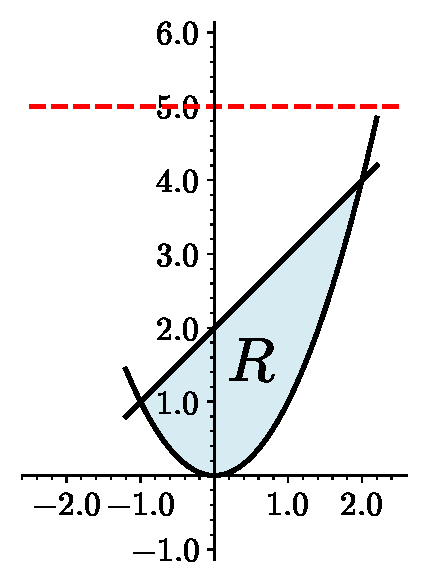
\includegraphics[scale=0.75]{plots/volume_by_slicing2_p1.pdf}
    \caption{Region between $y=x+2$ and $y=x^2$}
  \end{figure}
  
\begin{solutionorbox}[5.0in]

\end{solutionorbox}


\part $y=2$ and $y=\sqrt{x}$ about the line $x=-2$
  \begin{figure}[hbt!]\centering
    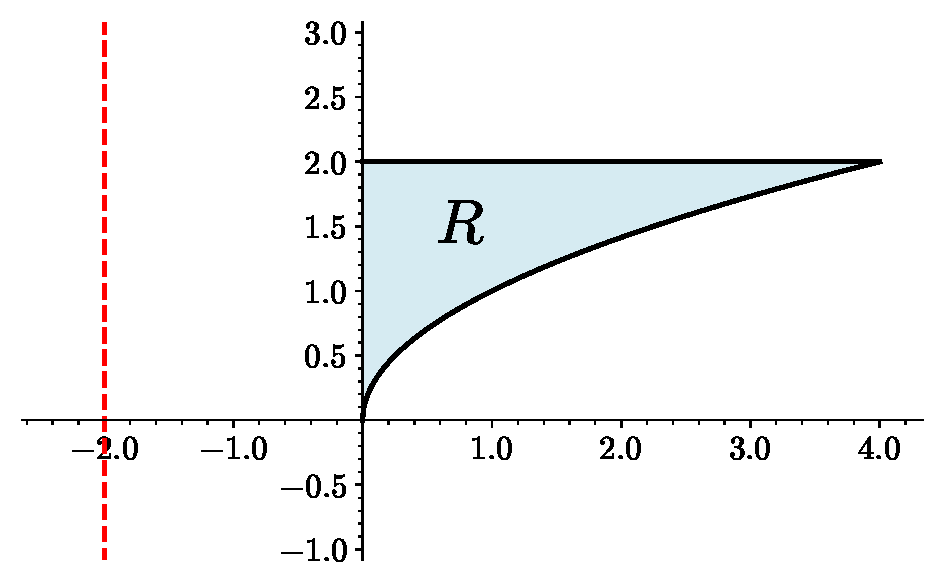
\includegraphics[scale=0.75]{plots/volume_by_slicing2_p2.pdf}
    \caption{Region between $y=2$ and $y=\sqrt{x}$}
  \end{figure}
\begin{solutionorbox}[6.0in]

\end{solutionorbox}

\end{parts}



\end{questions}\cleardoublepage

\section{Volumes by Shells}
\setcounter{figure}{0}
%asdf
\begin{questions}

\question Let $R$ be the region shown in the figure below.

\begin{parts}
\newcommand\answerboxlengthone{1.20in}

\part Draw an example of a shell created by revolving a Riemann rectangle at $x_k^*$ in the interval $[0,\sqrt{\pi}]$ about the $y$-axis.
\begin{figure}[hbt!]\centering
  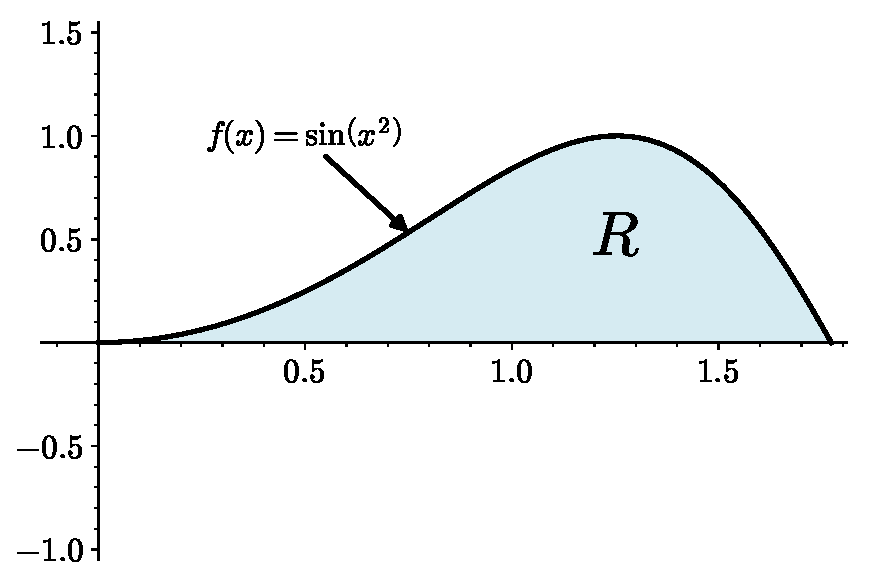
\includegraphics[scale=0.75]{plots/volume_by_shell_p1.pdf}
  \caption{Region bounded between $f(x)=\sin\lrp{x^2}$ and the $x$-axis}
\end{figure}

\part Draw the image that corresponds to unraveling the shell and label it.
\begin{solutionorbox}[\answerboxlengthone]
\end{solutionorbox}

\part What is the length of the shell?
\begin{solutionorbox}[\answerboxlengthone]
\end{solutionorbox}

\part What is the height of the shell?
\begin{solutionorbox}[\answerboxlengthone]
\end{solutionorbox}

\newpage 

\part What is the width of the shell?
\begin{solutionorbox}[\answerboxlengthone]
\end{solutionorbox}

\part Use this information to construct the Riemann sum that would calculate the volume of the solid of revolution.
\begin{solutionorbox}[\answerboxlengthone]
\end{solutionorbox}

\part Use your information from the previous part to construct and evaluate the definite integral that would calculate the volume of the solid of revolution.
\begin{solutionorbox}[4in]
\end{solutionorbox}

\end{parts}

\newpage
\question Let $R$ be the region shown in the figure below.

\begin{parts}
\newcommand\answerboxlengthone{1.20in}

\part Draw an example of a shell created by revolving a Riemann rectangle at $x_k^*$ in the interval $[0,2]$ about the line $x=3$.
\begin{figure}[hbt!]\centering
  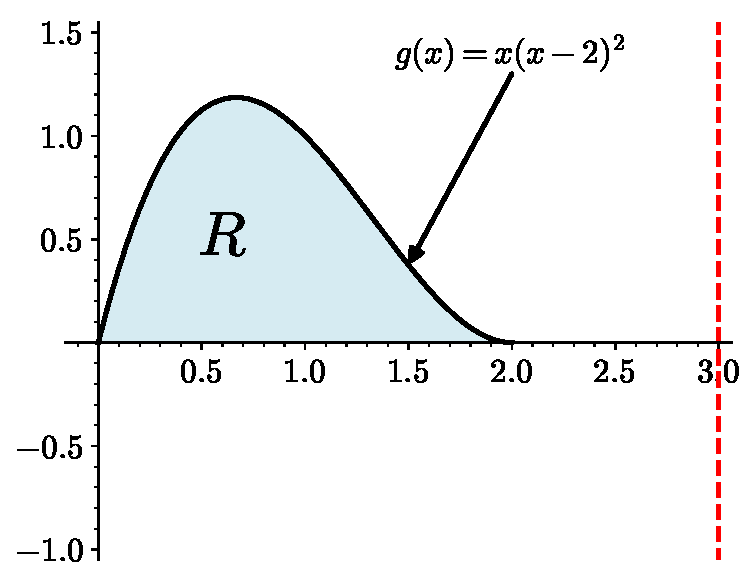
\includegraphics[scale=0.88]{plots/volume_by_shell_p2.pdf}
  \caption{Region bounded between $g(x)=x(x-2)^2$ and the $x$ axis}
\end{figure}

\part Draw the image that corresponds to unraveling the shell and label it.
\begin{solutionorbox}[\answerboxlengthone]
\end{solutionorbox}

\part What is the length of the shell?
\begin{solutionorbox}[\answerboxlengthone]
\end{solutionorbox}

\part What is the height of the shell?
\begin{solutionorbox}[\answerboxlengthone]
\end{solutionorbox}

\part What is the width of the shell?
\begin{solutionorbox}[\answerboxlengthone]
\end{solutionorbox}

\part Use this information to construct the Riemann sum that would calculate the volume of the solid of revolution.
\begin{solutionorbox}[\answerboxlengthone]
\end{solutionorbox}

\part Use your information from the previous part to construct and evaluate the definite integral that would calculate the volume of the solid of revolution.
\begin{solutionorbox}[4in]
\end{solutionorbox}

\end{parts}

\newpage
\question Find the volume of the solid created by rotating the region bounded by $y=x^2+2x-1$ and $y=2x$ about the line $x=-4$. Draw clearly labeled picture to support your answer.
\begin{solutionorbox}[9.25in]

\end{solutionorbox}

\question Find the volume of the solid created by rotating the region bounded by $y=\sin(x)+2$ and $y=\cos(x)$ on the interval $[0,\pi]$ about the line $x=6$.
\begin{solutionorbox}[9.25in]

\end{solutionorbox}



\end{questions}\cleardoublepage

\section{Arc Length and Surface Area}
\setcounter{figure}{0}
%asdf
\begin{questions}
\question Find the arc length of the specified function over the given domain.
\begin{parts}
\part $\displaystyle f(x)=x^2/2; \quad [0,\, 2]$
\begin{solutionorbox}[4.2in]
a
\end{solutionorbox}

\part $\displaystyle g(x)=\frac{1}{2}\lrp{e^x+e^{-x}}; \quad [0,\, \ln(5)]$
\begin{solutionorbox}[4.2in]

\end{solutionorbox}

\part $\displaystyle h(x)=\ln(\cos x); \quad [0,\, \pi/4]$
\begin{solutionorbox}[4.5in]

\end{solutionorbox}

\part $\displaystyle k(x)=\frac{1}{12}x^5+\frac{1}{5x^3}; \quad \left[\frac{1}{10},\, 1\right]$
\begin{solutionorbox}[4.5in]

\end{solutionorbox}

\end{parts}

\question Find the surface area of the described solid of revolution.
\begin{parts}
\part The solid formed by revolving $y=2x$ on $[0,2]$ about the $x$-axis.
\begin{solutionorbox}[4.4in]

\end{solutionorbox}

\part The solid formed by revolving $y=x^2$ on $[0,1]$ about the $y$-axis.
\begin{solutionorbox}[4.4in]

\end{solutionorbox}

\part The solid formed by revolving $y=\sqrt{x}$ on $[0,4]$ about the $x$-axis.
\begin{solutionorbox}[4.5in]

\end{solutionorbox}

\part The solid formed by revolving $y=\sqrt{a^2-x^2}$ on $[-a,a]$ about the $x$-axis.
\begin{solutionorbox}[4.5in]

\end{solutionorbox}

\end{parts}


\end{questions}\cleardoublepage

\section{Introduction to Sequences}
\begin{questions}
\question Consider the following sequence of number:
\[\{1, 3, 6, 10, 15, 21, \dots\}.\]
These are called \textit{triangular numbers} because they are the number of vertices as pictured below.
\begin{figure}[hbt!]
\centering
  
\includegraphics[scale=0.33]{plots/500px_First_six_triangular_numbers.png}
\caption{Triangular Numbers}
\end{figure}
\begin{parts}
  \part Write a \textit{recursive} definition for this sequence.
  \begin{solutionorbox}[0.75in]
    $T_{n+1}=T_n+n+1$ or $T_{n}=T_{n-1}+n$
  \end{solutionorbox}
  
  \part Find an \textit{explicit} formula for this sequence where $n=1$ is the first term of the sequence.
  \begin{solutionorbox}[1.0in]
    By looking at the pattern, we can observe the following:\\
    \begin{center}
      \begin{tabular}{l|l}
        $n$ & $T_n$ \\ \hline
        1   & 1\\
        2   & 1+2\\
        3   & 1+2+3\\
        $\vdots$ & $\vdots$ \\
        $n$ & $\displaystyle 1+2+\dots+n=\sum_{k=1}^n k$
      \end{tabular}
    \end{center}
    The sum of $k$ positive integers is given by the formula: $\frac{n(n+1)}{2}$, so $T_n=\frac{n(n+1)}{2}$.
  \end{solutionorbox}
  
  \part Determine what $T_{100}$ would be.
  \answerline[5050]
\end{parts}

\question Determine if the sequence has a least upper bound (supremum) and a greatest lower bound (infimum). If so, what are they?
\begin{parts}
\part \sequence{e^{-k}}{k=0}{\infty} \answerline[1]
\part \sequence{(-1)^kk}{k=0}{\infty} \answerline[DNE]
\part \sequence{3+\frac{1}{k^2+1}}{k=-\infty}{\infty} \answerline[3]
\end{parts}


\newpage

\question Match the formulas with the descriptions of the behavior of the sequence as $k$ goes to infinity. List the first five values in the sequence as justification of your answer.
\begin{parts}
  \begin{multicols}{3}
    \part \sequence{\frac{(-1)^n}{n+1}}{n=1}{\infty}\\[16pt]
    \part \sequence{\sin\left(\frac{1}{k}\right)}{k=1}{\infty}\\[16pt]
    \part \sequence{-4+\frac{(-1)^m}{m}}{m=0}{\infty}\\[16pt]
    \part \sequence{\frac{n\cos(n)}{2n+3}}{n=12}{\infty}\\[16pt]
    \part \sequence{n(n-1)-n}{n=-2}{\infty}\\[16pt]
    \part \sequence{-\frac{p!}{(p+1)!}}{p=0}{\infty}\\[16pt]
  \end{multicols}
\end{parts}

\begin{enumerate}[I.]
\item \numanswerline[D] Converges to $\frac{1}{2}$ from above and below.\vfill

\item \numanswerline[A] Converges to $0$ through positive numbers.\vfill

\item \numanswerline[B] Converges to $0$ from above and below.\vfill

\item \numanswerline[F] Converges to 0 through negative numbers.\vfill

\item \numanswerline[E] Diverges to $\infty$.\vfill

\item \numanswerline[C] Converges to $-4$ from above and below.\vfill
\end{enumerate}

\newpage

\question Opiates are drugs with a ``morphine-like pharmacological action" according to the Mayo Clinic \footnote{\url{https://www.mayomedicallaboratories.com/test-info/drug-book/opiates.html}}. Many of these drugs have a half-life of about 5 hours. Suppose a pharmaceutical company has developed a new synthetic opiate with a half-life of 6 hours.
\begin{parts}
\part Complete the following table to describe the first 24 hours after taking 20mg of the new synthetic opiate at 6 hour intervals.

\begin{table}[hbt!]\centering
  \begin{tabular}{l|c|c|c|c|c}
    hour           & 0 & 6 & 12 & 18 & 24 \\ \hline
    amount (mg)    & \myspace & \myspace & \myspace & \myspace & \myspace
  \end{tabular}
\end{table}

\begin{solution}
  \begin{center}
    \begin{tabular}{l|c|c|c|c|c}
      hour           & 0 & 6 & 12 & 18 & 24 \\ \hline
      amount (mg)    & 20 & 10 & 5 & 2.5 & 1.25
    \end{tabular}
  \end{center}
\end{solution}\vfill

\part Write an explicit equation that models this data of the form $N(t)=a_0(r)^{kt}$.
\begin{solutionorbox}[2.25in]
  $N(t)=20\left(\frac{1}{2}\right)^{t/6}=20\left(\sqrt[6]{\frac{1}{2}}\right)^{t}$
\end{solutionorbox}\vfill

\part What is the hourly decay rate of the drug?
\answerline[About 11\%]\vfill
\textit{}
\part As $t\to\infty$, what happens to the amount opiates?
\begin{solutionorlines}[1in]
The amount will tend towards zero.
\end{solutionorlines}\vfill


\end{parts}

\newpage

\question In this question, you will look at a sequence of functions, rather than a numerical sequence. Consider the function defined by $f_n(x)=\left(1+\frac{x}{n}\right)^n$ and the sequence defined by \sequence{f_n(x)}{n=0}{\infty}. Go to \url{https://www.desmos.com/calculator/wjwfifwfnn} to help with this question.
\begin{parts}
\part Below are the first 5 terms of this sequence of functions:
\[1\]
\[x+1\]
\[\frac{1}{4} x^{2} + x + 1\]
\[\frac{1}{27} x^{3} + \frac{1}{3} x^{2} + x + 1\]
\[\frac{1}{256} \, x^{4} + \frac{1}{16} \, x^{3} + \frac{3}{8} \, x^{2} + x + 1\]
What patterns or sequences of numbers do you notice?
\begin{solutionorbox}[1.75in]
  Answers will vary greatly. One possible answer is the fact that the leading coefficients (assuming $n\geq1$) is $n^n$.
\end{solutionorbox}\vfill

\part Use the Desmos graph that has been provided to record the different values of $f_n(1)$ to four decimal places.
\begin{table}[hbt!]\centering
  \begin{tabular}{c|c|c|c|c|c|c}
    $n$           & 0 & 1 & 10 & 100 & 1000 & $\infty$ \\ \hline
    $f_n(1)$    & \myspace & \myspace & \myspace & \myspace & \myspace & \myspace\\ \hline
    $f_n(2)$    & \myspace & \myspace & \myspace & \myspace & \myspace & \myspace
  \end{tabular}
\end{table}

\begin{solution}
\begin{center}
  \begin{tabular}{c|c|c|c|c|c|c}
    $n$           & 0 & 1 & 10 & 100 & 1000 & $\infty$ \\ \hline
    $f_n(1)$    & DNE & 2 & 2.594 & 2.705 & 2.171 & e \\ \hline
    $f_n(2)$    & DNE & 3 & 6.1717 & 7.2446 & 7.3743 & $e^2$
  \end{tabular}
\end{center}
\end{solution}


\vfill

\part What function do you hypothesize this sequence of functions converges to as $n\to\infty$? Give a justification of your answer. [Hint: $\lim_{n\to\infty}(1+1/n)^{n}=e$]
\begin{solutionorbox}[1.75in]
\[e^x\]
\end{solutionorbox}

\end{parts}

\newpage

\question Determine if the sequence is bounded or unbounded, then use an appropriate test to analyze the monotonicity of the given sequence.
\begin{parts}
\part \sequence{\frac{n}{n+3}}{n=0}{\infty}
\begin{solutionorbox}[2.5in]
We can use the Difference Test to show that this series is strictly increasing. 
\[\begin{aligned}
  a_{n+1}-a_n   &=\frac{n+1}{n+4}-\frac{n}{n+3} \\
                &=\frac{(n+1)(n+3)-n(n+4)}{(n+4)(n+3)} \\
                &=\frac{3}{(n+3)(n+4)}
\end{aligned}\]
So, $\forall_{n\geq0}a_{n+1}-a_n>0$; therefore, this sequence is strictly increasing. It is bounded below by 0 and above by 1.
\end{solutionorbox}

\part \sequence{\frac{k^3}{(k-1)!}}{k=0}{\infty}
\begin{solutionorbox}[2.5in]
Since we have a factorial in the problem, we should use the Ratio Test to determine the monotonicity. So, consider $\frac{a_{k+1}}{a_k}$.
\[\begin{aligned}
  \frac{a_{n+1}}{a_n}   &=\frac{(k+1)^3}{k!}\cdot\frac{(k-1)!}{k^3} \\
                        &=\frac{(k+1)^3}{k\cancel{(k-1)!}}\cdot\frac{\cancel{(k-1)!}}{k^3} \\
                        &=\frac{(k+1)^3}{k^4}
\end{aligned}\]
From this, we see that that this is converging to zero, which means it will be less than 1. However, it isn't less than 1 until $k\geq3$. Therefore, this sequence is eventually decreasing, bounded below by zero, and abounded above by 13.5.
\end{solutionorbox}

\part \sequence{e^{-k}k^3}{k=0}{\infty}
\begin{solutionorbox}[2.5in]
We'll use the First Derivative Test to show this is decreasing. First, we make the sequence continuous by making the function $a(x)=e^{-x}x^3$. Now, we take the derivative of $a(x)$: $a'(x)=x^2e^{-x}(3-x)$. Now, we'll create the sign chart.\\[4pt]

\begin{center}
\begin{tikzpicture}[]
  \draw[latex-latex,color=firstDerivative,line width=0.6mm] (-1,0)--(5,0); %edit for axis
  \foreach \x in  {0,3} % edit here for the vertical lines
  \draw[shift={(\x,0)},color=black] (0pt,3pt) -- (0pt,-3pt);
  \foreach \x in {0,3} % edit here for the numbers
  \draw[shift={(\x,0)},color=black] (0pt,0pt) -- (0pt,-3pt) node[below] {$\x$};
  
  %Insert Signs
  \node at (5.5,0pt) {$a'(x)$};
  \node at (1.5, 0.33) {$+$};
  \node at (4, 0.33) {$-$};
\end{tikzpicture}
\end{center}

So, $\forall_{x>3}a'(x)<0$, which means that $a(x)$ is decreasing after $x=3$. This, in return, means that the sequence is eventually decreasing, bounded above by $27e^{-3}$, and bounded below by 0.
\end{solutionorbox}
\end{parts}

\end{questions}\cleardoublepage

\section{The Integral Test}
For each of the following series, determine if the series converges or diverges. You must use a test or a well-known series (i.e. geometric or telescoping) to prove convergence AND divergence. If the series is geometric or telescoping, find the value to which the series converges.
\begin{questions}

\question $\serieswithstartnpk{1}{\infty}{\frac{1}{8^k}}$\seriesproof

\question $\serieswithstartnpk{1}{\infty}{\frac{8}{\sqrt{k}}}$\seriesproof

\question $\serieswithstartnpk{1}{\infty}{ \frac{7} }{ \sqrt[3]{k+1} }$\seriesproof

\vfill

\question $\serieswithstartnpk{1}{\infty}{ \frac{1}{\ln\lrp{5}^k} }$\seriesproof

\newpage

\question $\serieswithstartnpk{1}{\infty}{ k^2e^{-k} }$\seriesproof

\vfill

\question $\serieswithstartnpk{1}{\infty}{ \frac{3k}{k^2+4} }$\seriesproof

\newpage

\question Which of the following is required condition for applying the integral test to the sequence $\sequenceoverk{a_k}$, where $a_k=f(k)$.
\begin{enumerate}[I.]
  \item $f(k)$ is everywhere positive
  \item $f(k)$ is eventually monotonically decreasing
  \item $f(k)$ is eventually always continuous
\end{enumerate}

\begin{choices}
  \choice I only
  \choice II only
  \choice III
  \choice I \& II only
  \choice I \& III only
  \choice II \& III only
  \choice I, II, \& II
\end{choices}\vfill

\question Which of the following statements is false?
\begin{choices}
\choice $\seriesoverknp{\frac{1}{k^p}}$ converges if $p>1$ and diverges otherwise.
\choice If $\displaystyle a_k$ and $\displaystyle f(k)$ satisfy the requirements of the Integral Test, and if $\defintvarnp{1}{\infty}{f(k)}{k}$ converges, then $\serieswithstartnpk{1}{\infty}{a_k}=\defintvarnp{1}{\infty}{f(k)}{k}$.
\choice $\serieswithstartnpk{2}{\infty}{ \frac{1}{k\lrp{\ln k}^p} }$ converges if $p>1$.
\choice The integral test does not apply to divergent sequences.
\end{choices}\vfill

\question Which of the following sequences DO NOT meet the conditions of the Integral Test?
\begin{multicols}{3}
\begin{enumerate}[I.]
  \item $\sequenceoverk{k(\sin(k)+1)}$
  \item $\sequenceoverk{ \frac{1}{k^p+p} }$
  \item $\sequenceoverk{ \frac{1}{k\sqrt{k}} }$
\end{enumerate}
\end{multicols}

\begin{choices}
  \choice I only
  \choice II only
  \choice III only
  \choice I \& II only
  \choice I \& III only
  \choice II \& III only
  \choice I, II, \& II
\end{choices}\vfill





\end{questions}\cleardoublepage

\section{The Comparison Tests}
\begin{questions}
\question For each of the following, determine if the series converges or diverges, then use the direct comparison test to prove your answer.

\begin{parts}
  \part $\serieswithstartnpk{1}{\infty}{\frac{1}{2^k+k}}$\seriesproof
  \vfill
  
  \part $\serieswithstartnpvar{n}{1}{\infty}{\frac{1}{(n+1)^2}}$\seriesproof\vfill
  
  \newpage
  
  \part $\serieswithstartnpvar{\theta}{0}{\infty}{\frac{1+\cos(\theta)}{10^\theta}}$\seriesproof\vfill
  
  \part $\serieswithstartnpk{0}{\infty}{ \frac{k!}{(k+1)!} }$\seriesproof\vfill
\end{parts}

\newpage

\question For each of the following, determine if the series converges or diverges, then use the limit comparison test to prove your answer.

\begin{parts}
  \part $\serieswithstartnpk{1}{\infty}{ \frac{k-2}{k\sqrt{k}} }$\seriesproof\vfill
  
  \part $\serieswithstartnpvar{n}{1}{\infty}{ \frac{\sqrt[n]{e}}{n} }$\seriesproof\vfill
  
  \newpage
  
  \part $\serieswithstartnpvar{n}{1}{\infty}{ \frac{n!}{n^n} }$\seriesproof\vfill
  
  \part $\serieswithstartnpk{1}{\infty}{\frac{k^5}{k^6-2}}$\seriesproof\vfill
\end{parts}



\end{questions}\cleardoublepage

\section{The Ratio and Root Tests}
\begin{questions}
\question For each of the following, use the ratio test to determine if the series converges or diverges.

\begin{parts}
  \part $\serieswithstartnpk{1}{\infty}{ \frac{1}{k!} }$\seriesproof
  \vfill
  
  \part $\serieswithstartnpvar{n}{1}{\infty}{ \frac{3^n}{(n+1)!} }$\seriesproof\vfill
  
  \newpage
  
  \part $\serieswithstartnpvar{k}{0}{\infty}{ k^42^{-k} }$\seriesproof\vfill
  
  \part $\serieswithstartnpk{0}{\infty}{ \frac{\lrp{k!}^2}{(2k)!} }$\seriesproof\vfill
\end{parts}

\newpage

\question For each of the following, use the root test to determine if the series converges or diverges.

\begin{parts}
  \part $\serieswithstartnpk{1}{\infty}{ \lrp{\frac{k^2-2k+3}{7k^3+k-111}}^k }$\seriesproof\vfill
  
  \part $\serieswithstartnpvar{n}{1}{\infty}{ \lrp{1+\frac{ 2 }{ n } }^{n^2} }$\seriesproof\vfill
  
  \newpage
  
  \part $\serieswithstartnpvar{n}{1}{\infty}{ \lrp{\frac{n}{n+2}}^{3n^2} }$\seriesproof\vfill
  
  \part $\serieswithstartnpk{1}{\infty}{ \lrp{\sqrt[k]{k}-1}^{5k} }$\seriesproof\vfill
\end{parts}



\end{questions}\cleardoublepage

\section{Alternating Series Test}
\begin{questions}
\question For each of the following, determine if the series converges absolutely, conditionally, or diverges.

\begin{parts}
  \part $\serieswithstartnpk{0}{\infty}{ \frac{(-1)^k}{2k+1} }$\seriesproofabs
  \vfill

  \part $\serieswithstartpvar{n}{1}{\infty}{ (-1)^n\lrp{\frac{n}{3+n}}^n }$\seriesproofabs\vfill

  \newpage

  \part $\serieswithstartnpvar{k}{0}{\infty}{ \frac{(-1)^k}{k^2+10} }$\seriesproofabs\vfill

  \part $\serieswithstartpk{0}{\infty}{ (-1)^{k+1}\frac{\lrp{k!}^3}{(3k)!} }$\seriesproofabs\vfill

  \part $\serieswithstartpk{0}{\infty}{ (-1)^k\lrp{\frac{k^2-2k+3}{7k^3+k-111}} }$\seriesproofabs\vfill

  \part $\serieswithstartnpvar{n}{1}{\infty}{ \lrp{-\frac{1}{e}}^n }$\seriesproofabs\vfill

  \newpage

  \part $\serieswithstartnpvar{n}{1}{\infty}{ \frac{(-1)^{n+1}}{\ln(n)} }$\seriesproofabs\vfill

  \part $\serieswithstartnpk{0}{\infty}{ \lrp{-\frac{2k+\cos((k+1)\pi)}{k+1}}^k }$\seriesproofabs\vfill
\end{parts}
\end{questions}\cleardoublepage

\section{Convergence Test Review}
\begin{questions}
\question Give an example of a series that satisfies the given criteria.
\begin{parts}
  \part A series that is absolutely convergent.
  \begin{solutionorbox}[1in]
  \end{solutionorbox}
  
  \part A series that is conditionally convergent.
  \begin{solutionorbox}[1in]
  \end{solutionorbox}
  
  \part A series that is divergent, but the limit of the summand goes to zero.
  \begin{solutionorbox}[1in]
  \end{solutionorbox}
  
  \part An alternating series that DOES NOT contain $(-1)^k$. [Hint: think about your trigonometric functions.]
  \begin{solutionorbox}[1in]
  \end{solutionorbox}
\end{parts}

\question Explain why the series $\serieswithstartnpk{1}{\infty}{ \frac{\sqrt[k]{k}}{k} }$ is divergent.
\begin{solutionorlines}[1in]

\end{solutionorlines}

\newpage

\question Indicate if the given series converges or diverges by circling your choice. You must provide proof of your claim by correctly using one of the series tests.
\begin{parts}
\part $\serieswithstartnpk{1}{\infty}{ \frac{k}{3^k} }$ \hfill  {\Large \textsc{Converges / Diverges}}. \\[12pt]
  Proof\\[-0.35in]
  \begin{solutionorbox}[2.25in]

  \end{solutionorbox}

\part $\serieswithstartnpk{1}{\infty}{ \frac{\sqrt{k}}{k} }$ \hfill  {\Large \textsc{Converges / Diverges}}. \\[12pt]
  Proof\\[-0.35in]
  \begin{solutionorbox}[2.25in]

  \end{solutionorbox}
  
\part $\serieswithstartnpk{0}{\infty}{ \frac{1}{2^k+\sin(k)} }$ \hfill  {\Large \textsc{Converges / Diverges}}. \\[12pt]
  Proof\\[-0.35in]
  \begin{solutionorbox}[2.25in]

  \end{solutionorbox}
  %a
\newpage
  
\part $\serieswithstartnpk{0}{\infty}{ \frac{1\cdot4\cdot7\cdots(3k+1)}{100^k} }$ \hfill  {\Large \textsc{Converges / Diverges}}. \\[12pt]
  Proof\\[-0.35in]
  \begin{solutionorbox}[2.25in]

  \end{solutionorbox}
  
\part $\serieswithstartpk{1}{\infty}{ -2ke^{-k^2} }$ \hfill  {\Large \textsc{Converges / Diverges}}. \\[12pt]
  Proof\\[-0.35in]
  \begin{solutionorbox}[2.25in]

  \end{solutionorbox}
  
\part $\serieswithstartnpk{1}{\infty}{ \frac{(k+1)^k}{(2k)^k} }$ \hfill  {\Large \textsc{Converges / Diverges}}. \\[12pt]
  Proof\\[-0.35in]
  \begin{solutionorbox}[2.25in]

  \end{solutionorbox}
\end{parts}

\newpage

\question Indicate if the given series converges absolutely, converges conditionally, or diverges. Prove your claim.
\begin{parts}
  \part $\serieswithstartnpk{1}{\infty}{ \frac{(-2)^k}{1+3^k} }$ \hfill  {\Large \textsc{Absolutely / Conditionally / Diverges}}. \\[12pt]
  Proof\\[-0.35in]
  \begin{solutionorbox}[3.5in]

  \end{solutionorbox}
  
\part $\serieswithstartpk{1}{\infty}{ (-1)^k\frac{\sqrt{k}}{3k-1} }$ \hfill  {\Large \textsc{Absolutely / Conditionally / Diverges}}. \\[12pt]
  Proof\\[-0.35in]
  \begin{solutionorbox}[3.5in]

  \end{solutionorbox}

\end{parts}



\end{questions}


\cleardoublepage
\end{document}